\documentclass[dvipdfmx]{jsarticle}
\usepackage[T1]{fontenc}                                                       
\usepackage{lmodern}                                                           
\usepackage{latexsym}                                                          
\usepackage{amsfonts}                                                          
\usepackage{amssymb}                                                           
\usepackage{mathtools}                                                         
\usepackage{amsthm}                                                           
\usepackage{multirow}     
\usepackage{graphicx}
\usepackage{wrapfig}
\usepackage{here}

\title{発展プログラミング レポート 第三回}
\author{5417055 杉山輝晃}
\date{\today}



\begin{document}
\maketitle
\section{概要}
このレポートは発展プログラミング第三回、ネットワークプログラミングを活かしたプログラムを制作し、その詳細についてまとめたものである。

\section{制作内容}
簡易色相検定アプリ。

serverclientを立ち上げるとclient側の画面に問題と対象の色のついた円が表示され、中心にならぶ色のついた円から題意にそった色のついた円をクリックする。「正解」と「不正解」が表示される。

\section{プログラム動作}
server側のプログラム。clientと接続するとランダムに生成したHSBのcolorと問題を選ぶためのqsをString型にして連結し、serverに渡している。

\begin{verbatim}
import processing.net.*;

Server server;

void setup() {
  server = new Server(this, 5204);
  //size(600,600);
}

void draw() {
  
}

void clientEvent(Server ss,Client client){
  println("Re connected");
  println("First!");
  String h = str((int (random(360))));
  String s = str((int (random(60,100))));
  String b = str((int(random(50,100))));
  String hsb = h + ',' + s + ',' + b +',';
  int qs = 0;//int(random(4));
  hsb += str(qs);
  println(hsb);
  ss.write(hsb); 
  println("come");
}
void serverEvent(Server ss,Client client){
  println("connected");
  println("First!");
  String h = str((int (random(360))));
  String s = str((int (random(60,100))));
  String b = str((int(random(50,100))));
  String hsb = h + ',' + s + ',' + b +',';
  int qs = int(random(4));
  hsb += str(qs);
  println(hsb);
  ss.write(hsb); 
}
\end{verbatim}

client側のプログラム。
serverと接続し、読み込まれたStringを分割しcolor型に置き直す。qIdに入った値によってq配列内の問題文が決まる。colorCalcでは同系色や補色などの計算を行っている。同系色では彩度明度を変える、同一トーンでは彩度明度を変えず色相を変える、隣接色は色相に一定の値の変化を与える、補色はRGB値に直し、それぞれの値を比較し最大値を計算。最大値から各RGB値を引いた値をcolor型にする。



\begin{verbatim}
import processing.net.*;

class Button {
  int cx, cy, size;
  color fillColor;
  boolean selected = false;
  int id;
  Button(int cx, int cy, int size, color fillColor, int id) {
    //this.hand = hand;
    this.cx = cx;
    this.cy = cy;
    this.size = size;
    this.fillColor = fillColor;
    this.id = id;
  }

  int getId() {
    return this.id;
  }

  boolean clicked() {
    return dist(mouseX, mouseY, cx, cy) <= size / 2;
  }

  void draw() {
    colorMode(HSB, 360, 100, 100);
    noStroke();
    if (!this.selected) {
      fill(this.fillColor);
    } else {
      color pushed = color(int(round(hue(this.fillColor))), int(round(saturation(this.fillColor))), int(round(brightness(this.fillColor)))-20 );
      fill(pushed);
    }
    ellipse(this.cx, this.cy, this.size, this.size);
    fill(0);
    textAlign(CENTER, CENTER);
    //text("word",this.cx, this.cy);
  }
}

Client client;
//Status currentStatus = Status.INPUT;
Button[] buttons;
//Hand enemy = null;

void setup() {
  size(400, 400);

  client = new Client(this, "127.0.0.1", 5204);
  colorMode(HSB, 360, 100, 100);
  //int size = 100;
  buttons = new Button[3];
}


String[] q = {"同系色", "同一トーン", "隣接色", "補色", "対象色"};
int qId = -1;
int corId = -1;
int size = 100;
void draw() {
  background(0, 0, 100);
  if (qId != -1) {
    text(q[qId]+"は?", width/2, height*2/3, 200);
    fill(temp);
    ellipse(width/2, height*3/4, 30, 30);
    if (buttons[0]!=null) {
      int correct = -1;
      //Hand hand = null;
      //clientEvent(client);

      for (int i = 0; i < 3; i++) {
        buttons[i].draw();
        if (buttons[i].selected) {
          correct = buttons[i].getId();
        }
      }
      if (correct!=-1) {
        if (correct == corId) {
          text("正解!!", width/2, height/3, 200);
        } else {
          text("不正解", width/2, height/3, 200);
        }
      }
    }
  }
}


void mouseClicked() {
  //client.write(123);
  //if (currentStatus == Status.INPUT) {
  int selected = -1;
  for (Button button : buttons) {
    if (button.clicked()) {
      selected = button.getId();
      button.selected = true;
      println("clicked:"+selected);/////////////////////////
    }
  }
  if (selected != -1) {
    //client.write(selected);
    //println("send to server");//////////////////////////////
    selected = -1;
    //currentStatus = Status.WAIT;
  }
  /*} else if (currentStatus == Status.RESULT) {
   for (Button button : buttons) {
   button.selected = false;
   }
   enemy = null;
   currentStatus = Status.INPUT;
   }*/
}
String[] xy;
color temp;
void clientEvent(Client client) {
  while (client.available() > 0) {
    xy = split(client.readString(), ',');
    println('(' + xy[0] + " , " +xy[1] + " , " + xy[2] + ")" + xy[3]);
  }
  buttons[0] = new Button(size / 2, height / 2, size, color(int(random(360)), int(random(20, 90)), int(random(20, 90))), 0);
  buttons[1] = new Button(width / 2, height / 2, size, color(int(random(360)), int(random(20, 90)), int(random(20, 90))), 1);
  buttons[2] = new Button(height-size / 2, height / 2, size, color(int(random(360)), int(random(20, 90)), int(random(20, 90))), 2);
  qId = int(xy[3]);//text(q[int(xy[3])],width/3,height/5,100);
  temp = color(int(xy[0]), int(xy[1]), int(xy[2]));
  colorCalc(temp, qId);
}

void colorCalc(color sorce, int id) {
  colorMode(HSB);
  int correct = int(random(3));
  corId = correct;
  int position;
  if (correct == 0) {
    position = size/2;
  } else if (correct == 1) {
    position = width/2;
  } else {
    position = height-size/2;
  }
  println("correct is " + correct);
  if (id == 0) {//同系色
    buttons[correct] = new Button(position, height / 2, size, color(int(round(hue(sorce))), int(random(40, 90)), int(random(40, 90))), correct);
  } else if (id == 1) {//同一トーン
    buttons[correct] = new Button(position, height / 2, size, color(int(random(360)), int(saturation(sorce)), int(brightness(sorce))), correct);
  } else if (id == 2) {//隣接色
    int temp = int(random(2));
    if (temp==0) {temp=15;} else {temp=-15;}
    buttons[correct] = new Button(position, height / 2, size, color(int(round(hue(sorce))) + temp,int(saturation(sorce)), int(brightness(sorce))) , correct);
  } else if (id == 3) {//補色
    colorMode(RGB);
    int r = (int)red(sorce);
    int g = (int)green(sorce);
    int b = (int)blue(sorce);
    int max = max(r,g,b);
    color temp = color(max-r,max-g,max-b);
    buttons[correct] = new Button(position, height / 2, size, temp, correct);
  } else if (id == 4) {//対象色
    colorMode(RGB);
    int r = (int)red(sorce);
    int g = (int)green(sorce);
    int b = (int)blue(sorce);
    int max = max(r,g,b);
    color temp = color(max-r,max-g,max-b);
    int t = int(random(2));
    if (t==0) {t=15;} else {t=-15;}
    colorMode(HSB);
    
    buttons[correct] = buttons[correct] = new Button(position, height / 2, size, color(int(round(hue(temp))) + t,int(saturation(temp)), int(brightness(temp))) , correct);
  } else {
    println("ERORR!!");
    exit();
  }
}
\end{verbatim}

\section{}
\begin{figure}
  \centering
  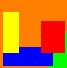
\includegraphics[width=5cm]{s.jpeg}
  \caption{s.jpeg}
\end{figure}


\section{工夫した点}
前回前々回と色相に関するプログラムを制作していたため今回もそのテーマを一貫することとした。このプログラムで5問の色相に関する問題を体験することができる。ランダムなbuttonを最初に3つ描画し、その上から正解の色のついたbuttonを描画することで位置をランダムにすることができた。正解の番号とbuttonクリックで得られるIdが一致すれば正解となる。プログラムの再起動をしなくても何度も遊べるものにしたかったが、serverとの再接続等の処理が何度試行しても実装できなかったため、このプログラムは1問のたびに再起動する必要がある。
\end{document}


